\begin{frame}{Traitement acoustique : extraction de paramètres}
	\begin{itemize}
	\item MFCC(Mel Frequency Cepstral Coeficients)
	\item LPCC(Linear Predictive Cepstral Coeficients)
	\item PLP(Perceptuqal Linear Predictive analysis)
	\end{itemize}
\end{frame}


\begin{frame}{MFCC}

\begin{figure}
\centering
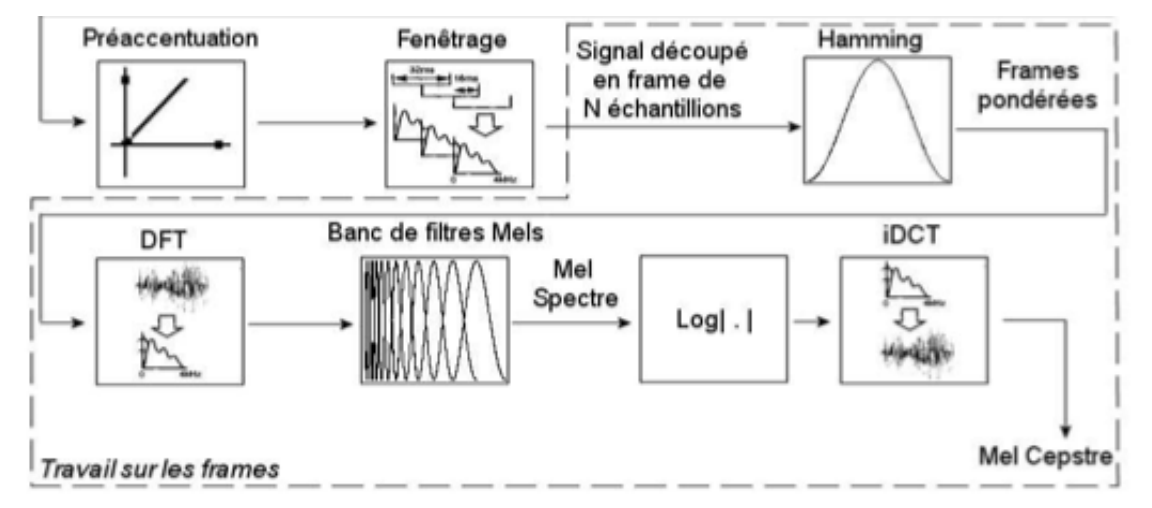
\includegraphics[width=8cm]{images/schema_MFCC.png}
\caption{Schéma de MFCC}
\end{figure}
\end{frame}

\begin{frame}{MFCC}
\begin{itemize}
\item Préaccentuation du signal
\item Découpage du signal en fenêtre
\item Application d’une fenêtre de Hamming
\item Création du banc de filtres
\item Conversion en échelle de mel
\item Application d’une DCT (Discrete Cosinus Transform) sur les portions
\end{itemize}
\end{frame}

\begin{frame}{Décodage acoustique et apprentissage}

\begin{itemize}
\item Chaînes et modèles de Markov cachés  
\item Critère du maximum de vraisemblance
\item Critère de Viterbi
\end{itemize}

\end{frame}

\begin{frame}{Adaptation}
\begin{block}{Méthode MLLR}
La méthode MLLR qui signifie Maximum Likelihood Linear Regression permet d’adapter des modèles acoustiques par régression linéaire.
\end{block}
\begin{block}{Méthode MAP}
La méthode MAP pour estimation du Maximum à postériori est une méthode bayésienne. Elle permet de modifier les paramètres d’un modèle générique pour se rapprocher des données de test.
\end{block}

\end{frame}

\begin{frame}{Création du Modèle acoustique en utilisant Sphinxtrain}
Les données d'entrées sont composés, entre autre:
\begin{itemize}
\item d'un ensemble de fichiers acoustiques(corpus).
\item d'un fichier de transcription qui contient l'ensemble de mots prononcés pour chaque enregistrement(fichier acoustique).
\item d'un fichier qui définie la liste des phonèmes utilisées.
\end{itemize}
\end{frame}